\documentclass{report}
\usepackage{csquotes}
\usepackage{float}
\usepackage{graphicx}
\usepackage[italian]{babel}
\usepackage[a4paper,margin=2.5cm]{geometry}
\usepackage[hidelinks]{hyperref}
\usepackage[
backend=biber,
style=ieee,
sorting=none,
]{biblatex}
\usepackage{xcolor}
\usepackage{listings}

% Define CMake language
\lstdefinelanguage{CMake}{
  keywords={
    add_executable, add_library, target_link_libraries,
    target_include_directories, project, cmake_minimum_required,
    set, if, endif, else, elseif, foreach, endforeach,
    while, endwhile, function, endfunction, macro, endmacro,
    include, find_package, message, option,
    install, file, configure_file,
    target_compile_definitions,
    target_compile_options,
    target_sources,
    enable_testing,
    add_test
  },
  sensitive=true,
  morecomment=[l]{\#},
  morestring=[b]",
}

% Define style
\lstdefinestyle{cmake}{
  language=CMake,
  basicstyle=\ttfamily\small,
  keywordstyle=\color{blue}\bfseries,
  commentstyle=\color{gray}\itshape,
  stringstyle=\color{green!50!black},
  numbers=left,
  numberstyle=\tiny\color{gray},
  stepnumber=1,
  numbersep=10pt,
  backgroundcolor=\color{black!2},
  showspaces=false,
  showstringspaces=false,
  showtabs=false,
  frame=single,
  rulecolor=\color{black!20},
  tabsize=2,
  breaklines=true,
  breakatwhitespace=true,
  captionpos=b,
  columns=fullflexible
}

\title{Report primo progetto di Metodi del calcolo scientifico}
\author{Daniele Besozzi 894998 \\ Andrea Consonni 900116 \\ Matteo Cervini 902225}
\date{\today}

\addbibresource{bibliography.bib}

\begin{document}
\maketitle

\tableofcontents
\chapter{Presentazione degli ambienti}
Le misure effettuate per questo progetto sono state eseguite su una macchina con le seguenti caratteristiche:
\begin{itemize}
	\item Processore: AMD ryzen 7 5700G (8 core, 16 thread, 3.8 GHz)
	\item RAM: 32 GB DDR4 3200 MHz
	\item Sistemi operativi: Windows 11 25H2 e Linux Fedora 44
	\item Linguaggi di programmazione: C++ e Matlab
	\item Dischi: SSD NVMe 
\end{itemize}
\section{Matlab}
Per quanto riguarda Matlab, abbiamo utilizzato la versione R2025b.
Per la risoluzione dei sistemi di equazioni è stato utilizzato il comando \texttt{mldivide}, che implementa una serie di controlli per scegliere il metodo più adatto a seconda del tipo di matrice (densa, sparsa, simmetrica, ecc.).
\begin{figure}
	\centering
	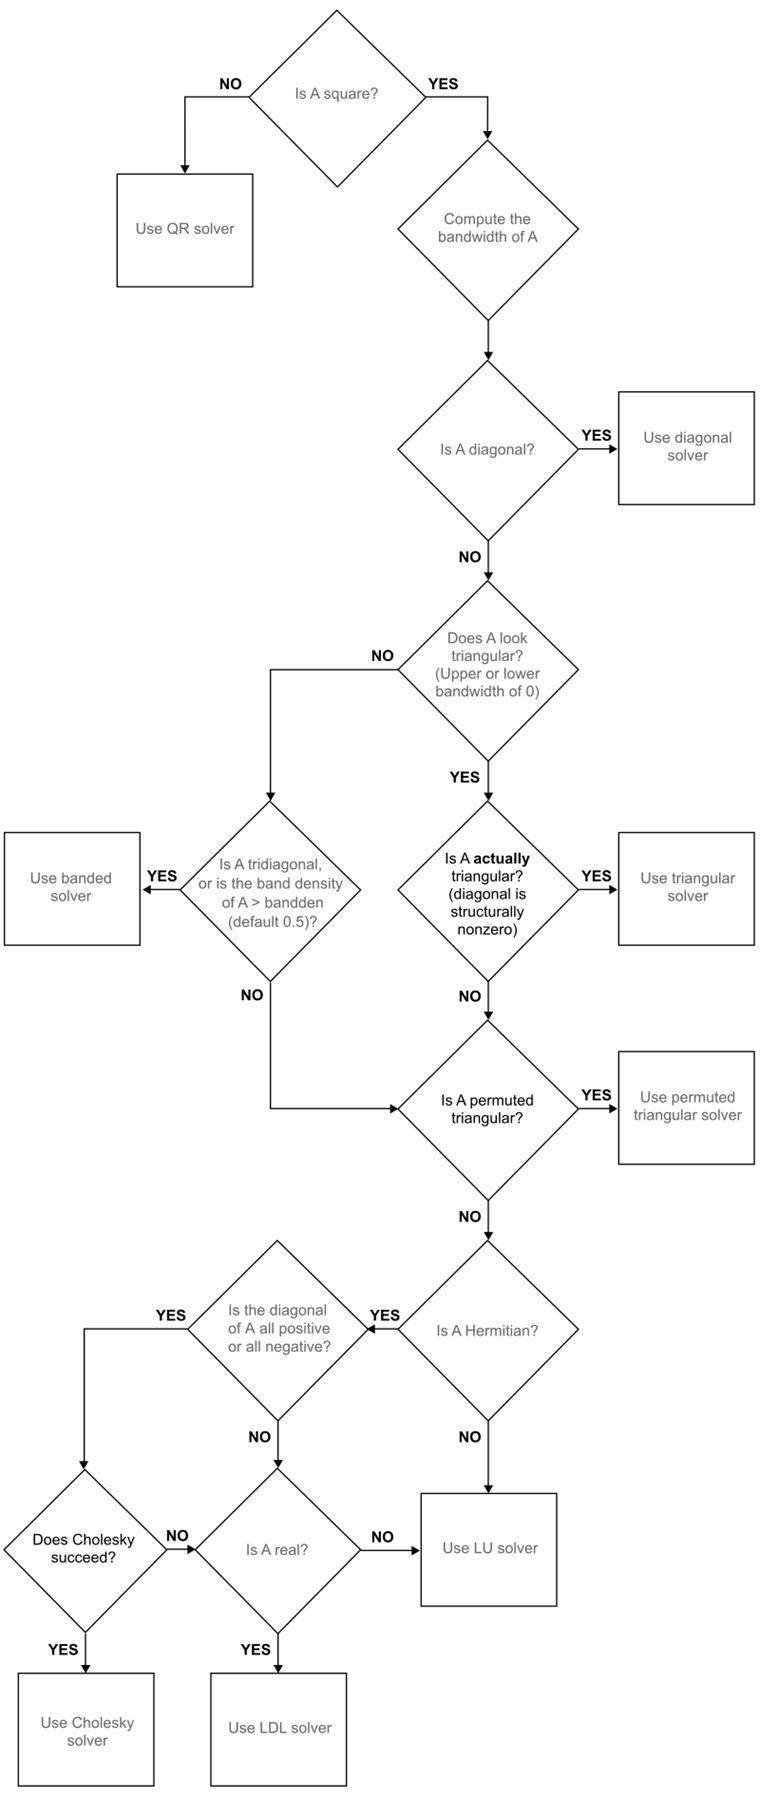
\includegraphics[height=0.95\textheight]{figures/mldivide_sparse.png}
	\caption{Scelta del metodo di risoluzione in Matlab per matrici sparse di \texttt{mldivide} \cite{noauthor_mldivide_nodate}.}
	\label{fig:mldivide_sparse}
\end{figure}
Questa libreria viene mantenuta e aggiornata regolarmente da MathWorks, ottimizzando i metodi di risoluzione per alcuni tipi di matrici	e migliorando le prestazioni complessive.
La documentazione ufficiale di Matlab fornisce i dettagli sulla selezione del metodo di risoluzione in base alle caratteristiche della matrice, dividendo in due macro categorie: matrici dense e matrici sparse.
In particolare, in figura~\ref{fig:mldivide_sparse} possiamo vedere il processo di selezione del metodo di risoluzione per matrici sparse, che è quello che abbiamo utilizzato per i nostri benchmark.
\section{C++}
Per quanto riguarda C++, abbiamo scelto di utilizzare la libreria \texttt{Eigen}, la quale mette a disposizione
una vasta gamma di funzioni per l'algebra lineare, come per la manipolazione di matrici e vettori oppure per la risoluzione
di sistemi di equazioni lineari.
Eigen permette inoltre di interfacciarsi con diversi moduli esterni per la risoluzione  di sistemi di equazioni lineari, come, ad esempio, il pacchetto SuiteSparse,
il quale è stato utilizzato per i benchmark presentati in questo report.
In particolare, abbiamo utilizzato la libreria \texttt{CHOLMOD} di SuiteSparse, la quale offre un metodo di risoluzione tramite fattorizzazione di Cholesky più efficiente rispetto al risolutore standard con metodo di Cholesky offerto da Eigen \cite{eigen_simpicial_llt}. 
L'interfaccia di Eigen per \texttt{CHOLMOD}, contenuta nel modulo \texttt{CholmodSupport} \cite{cholmod_eigen}, permette di sfruttare le diverse funzionalità offerte dalla libreria.
\subsubsection{CHOLMOD}
\texttt{CHOLMOD} è una libreria che permette di svolgere efficientemente diverse operazioni su matrici sparse.
In particolare, la libreria offre funzioni per la fattorizzazione di matrici sparse, simmetriche e definite positive
tramite il metodo di Cholesky e per la risoluzione di sistemi lineari. La libreria è scritta nel linguaggio di programmazione C.
Sia $A$ una matrice sparsa, simmetrica e definita positiva; allora la sua decomposizione ottenuta usando il metodo di Cholesky è $A = LL^T$,
con $L$ una matrice triangolare inferiore. 
\texttt{CHOLMOD} implementa due tipi di risolutori di sistemi di equazioni lineari sparsi che sfruttano questa decomposizione:
uno \textbf{supernodale} e uno \textbf{non-supernodale} \cite{chen_algorithm_2008}.
In particolare, abbiamo scelto di utilizzare l'implementazione \textbf{supernodale} dell'algoritmo di risoluzione, il quale è accessibile in Eigen costruendo un risolutore della classe \texttt{CholmodSupernodalLLT}\cite{supernodal_chol_eigen}.
%Informalmente, data le decomposizione di Cholesky $A = LL^T$, un \textbf{supernodo} è un insieme di colonne adiacenti di $L$ aventi un pattern identico di entrate non nulle.
%I supernodi sono tipicamente immagazzinati in memoria in modo tale da sfruttarne la struttura, come, per esempio, in matrici dense di dimensioni $s \times z$, dove
%$s$ è il numero di entrate non nulle nella prima colonna del supernodo e $z$ è il numero di colonne nel supernodo \cite{davis_dynamic_2009}.
Gli algoritmi supernodali si basano sulla decomposizione della matrice $A$ in termini di blocchi di colonne, chiamati \textbf{supernodi}. L'algoritmo implementato da CHOLMOD è composto da tre fasi di calcolo principali:
\begin{enumerate}
	\item La prima analizza la struttura della matrice e riordina le righe e le colonne per minimizzare il fill-in, ovvero l'introduzione di elementi non-nulli in $L$ che non compaiono nella posizione corrispondente in $A$.
	Il riordinamento della matrice è un'importante fattore di performance, dato che con meno valori non nulli il numero di operazioni necessario e il peso in memoria diminuisce.
	\item La seconda fase fattorizza la matrice applicando operazioni sui supernodi
	\item La terza risolve due sistemi triangolari di equazioni: $Ly = b$ e $L^T x = y$ nel caso della fattorizzazione di Cholesky.
\end{enumerate}
Tra le tre fasi, quella di fattorizzazione rappresenta la parte computazionalmente più onerosa del risolutore implementato da CHOLMOD \cite{le_fevre_selective_2022}.
Per sfruttare al meglio le moderne architetture delle CPU multicore, \texttt{CHOLMOD} utilizza la libreria \texttt{Open MultiProcessing (OpenMP)} \cite{cholmod_doc} per implementare la parallelizzazione di alcune delle operazioni necessarie alla risoluzione del sistema di equazioni lineari,
permettendo quindi di sfruttare al meglio la CPU e, agli scopi del benchmark, ottenere un confronto più equo con Matlab.
Infine, \texttt{CHOLMOD} dipende inoltre da diverse librerie per effettuare i calcoli necessari alla decomposizione e alla risoluzione del sistema di equazioni lineari:
\begin{itemize}
	\item \textbf{Librerie per l'ordinamento della matrice}: Per effettuare l'ordinamento della matrice nella prima fase dell'algoritmo di risoluzione, \texttt{CHOLMOD} può utilizzare diversi algoritmi, come \textit{Approximate Minimum Degree ordering} e \texttt{METIS} \cite{le_fevre_selective_2022}.
	Per questo motivo, \texttt{CHOLMOD} dipende dalle librerie di SuiteSparse \texttt{AMD, CAMD, COLAMD, CCOLAMD} e \texttt{METIS}.
	\item \textbf{Basic Linear Algebra Subroutines (BLAS)}: BLAS \cite{blas_doc} è un insieme di specifiche open per l'implementazione di funzioni a basso livello per svolgere le comuni operazioni richieste per l'algebra lineare.
	Esistono diverse implementazioni delle funzioni descritte da BLAS, tra cui \textbf{OpenBLAS} e \textbf{FlexiBLAS}, entrambe utilizzate per i benchmark presentati in questo report.
	\item \textbf{Linear Algebra PACKage (LAPACK)}: LAPACK \cite{lapack_doc} è una libreria che offre diverse funzioni per la risoluzione di sistemi lineari. La libreria dipende dalla presenza di un'implementazione di BLAS ed è scritta
	in modo tale che la computazione sia svolta effettuando il più possibile chiamate alle funzioni offerte dall'implementazione di BLAS sottostante.
\end{itemize}
\section{Windows}

\section{Linux}













\chapter{Tempo di esecuzione}
\section{Modalità di misurazione}
Per effettuare le misurazioni sul tempo di risoluzione del sistema, abbiamo utilizzato le funzionalità offerte nativamente dai
rispettivi linguaggi:
\begin{itemize}
    \item \textbf{Matlab}: abbiamo utilizzato i comandi \texttt{tic} e \texttt{toc} per rispettivamente far partire il timer
    e fermarlo.
    \item \textbf{C++}: per effettuare la misurazione, il programma C++ calcola la differenza di tempo da poco dopo aver letto la matrice in memoria
    a subito dopo la risoluzione del sistema. Per ottenere i due istanti di tempo necessari al calcolo, abbiamo utilizzato la funzione \texttt{std::chrono::high\_resolution\_clock::now()}
    della libreria \texttt{chrono} del linguaggio.
\end{itemize}

\lstinputlisting[
    language=C++,
    style = Cpp-editor,
    firstline = 105,
    lastline = 133,
    firstnumber = 105,
    caption = Porzione del codice C++ in cui si calcola il tempo di esecuzione
]{../cpp/utils/utils.hpp}
\clearpage
\lstinputlisting[
    style=Matlab-editor,
    firstline=66,
    lastline=72,
    firstnumber=66,
    caption = Porzione del codice Matlab in cui si calcola il tempo di esecuzione
]{../matlab/main.m}
\section{Risultati}





\chapter{Utilizzo della memoria}
\section{Misura utilizzata}
Poiché Linux e Windows offrono statistiche diverse riguardanti la memoria allocata per un processo, è stato
necessario utilizzare due metriche di memoria diverse:
\begin{itemize}
    \item \textbf{Linux}: Per Linux abbiamo utilizzato la misura \textbf{Resident Set Size} (RSS), la quale indica la memoria effettivamente occupata 
    \item \textbf{Windows}:  
\end{itemize}





\section{Profiling della memoria}
Per effettuare le misurazioni sullo spazio occupato in memoria dei due programmi sviluppati,
è stato necessario scrivere due ulteriori programmi distinti, uno per Windows e uno per Linux, per il campionamento della memoria occupata da un
determinato processo.
Questa necessità nasce da problematiche legate sia a Matlab che a C++.
Per quanto riguarda Matlab, la pressoché inesistente documentazione sul profiler integrato nell'ambiente di sviluppo \cite{mathworks_profiling}
rende particolarmente arduo comprendere appieno la misurazione ottenuta. 
Per C++, invece, non abbiamo trovato un profiler agnostico al sistema operativo che indicasse la quantità di memoria utilizzata per ogni chiamata
ad una certa funzione (nel nostro caso, la funzione \texttt{calculate\_benchmark()}).
Di seguito, riportiamo i due programmi scritti. I linguaggi utilizzati sono \textbf{Powershell} per Windows e \textbf{Bash} per Linux.

\lstinputlisting[
    language=Powershell,
    style = PowerShell-editor,
    caption = Sampler scritto per Windows in Powershell
]{../profilers/mem_sampler.ps1}
\clearpage
\lstinputlisting[
    language=Bash,
    style = Bash-editor,
    caption = Sampler scritto per Linux in Powershell
]{../profilers/mem_sampler.sh}
\chapter{Precisione delle soluzioni}
\section{Misura utilizzata}
Per misurare l'errore relativo abbiamo utilizzato la formula fornita dalla traccia:
$$\textrm{errore relativo } = \frac{||x - xe||_2}{||xe||_2}$$
dove, dati $A \in \mathbb{R}^{n \times n}$ e $xe \in \mathbb{R}^n$ con $xe = [1, 1, 1, \dots, 1]$, 
calcoliamo il termine noto del sistema $Ax = b$ come $b = A \cdot xe$. 
Il vettore $x$ è ottenuto risolvendo il sistema di equazioni $Ax = b$.
La risoluzione del sistema in C++ e in Matlab è già stata mostrata rispettivamente ai listings \ref{lst:execution-time-cpp} e \ref{lst:execution-time-matlab}.
\section{Analisi dei risultati}
Le misurazioni ottenute per entrambi i programmi su piattaforma Windows e su Linux sono riportate rispettivamente in figura \ref{fig:windows_relerr} 
e \ref{fig:linux_relerr}. Il confronto delle misurazioni ottenute per tutti i sistemi operativi è invece riportato in figura \ref{fig:complete_relerr}. Come si può evincere
dai grafici, la misura dell'errore relativo non dipende dal sistema operativo su cui si eseguono i programmi, ma solamente dal linguaggio e dalle librerie o funzionalità utilizzate.
Seppur gli errori registrati differiscono marginalmente tra i due linguaggi, si è registrato mediamente un errore relativo minore su C++ rispetto a Matlab, con una sola delle matrici
di ordine più elevato che ha registrato un errore relativo maggiore su C++ rispetto a Matlab.
\begin{figure}[H]
    \centering
    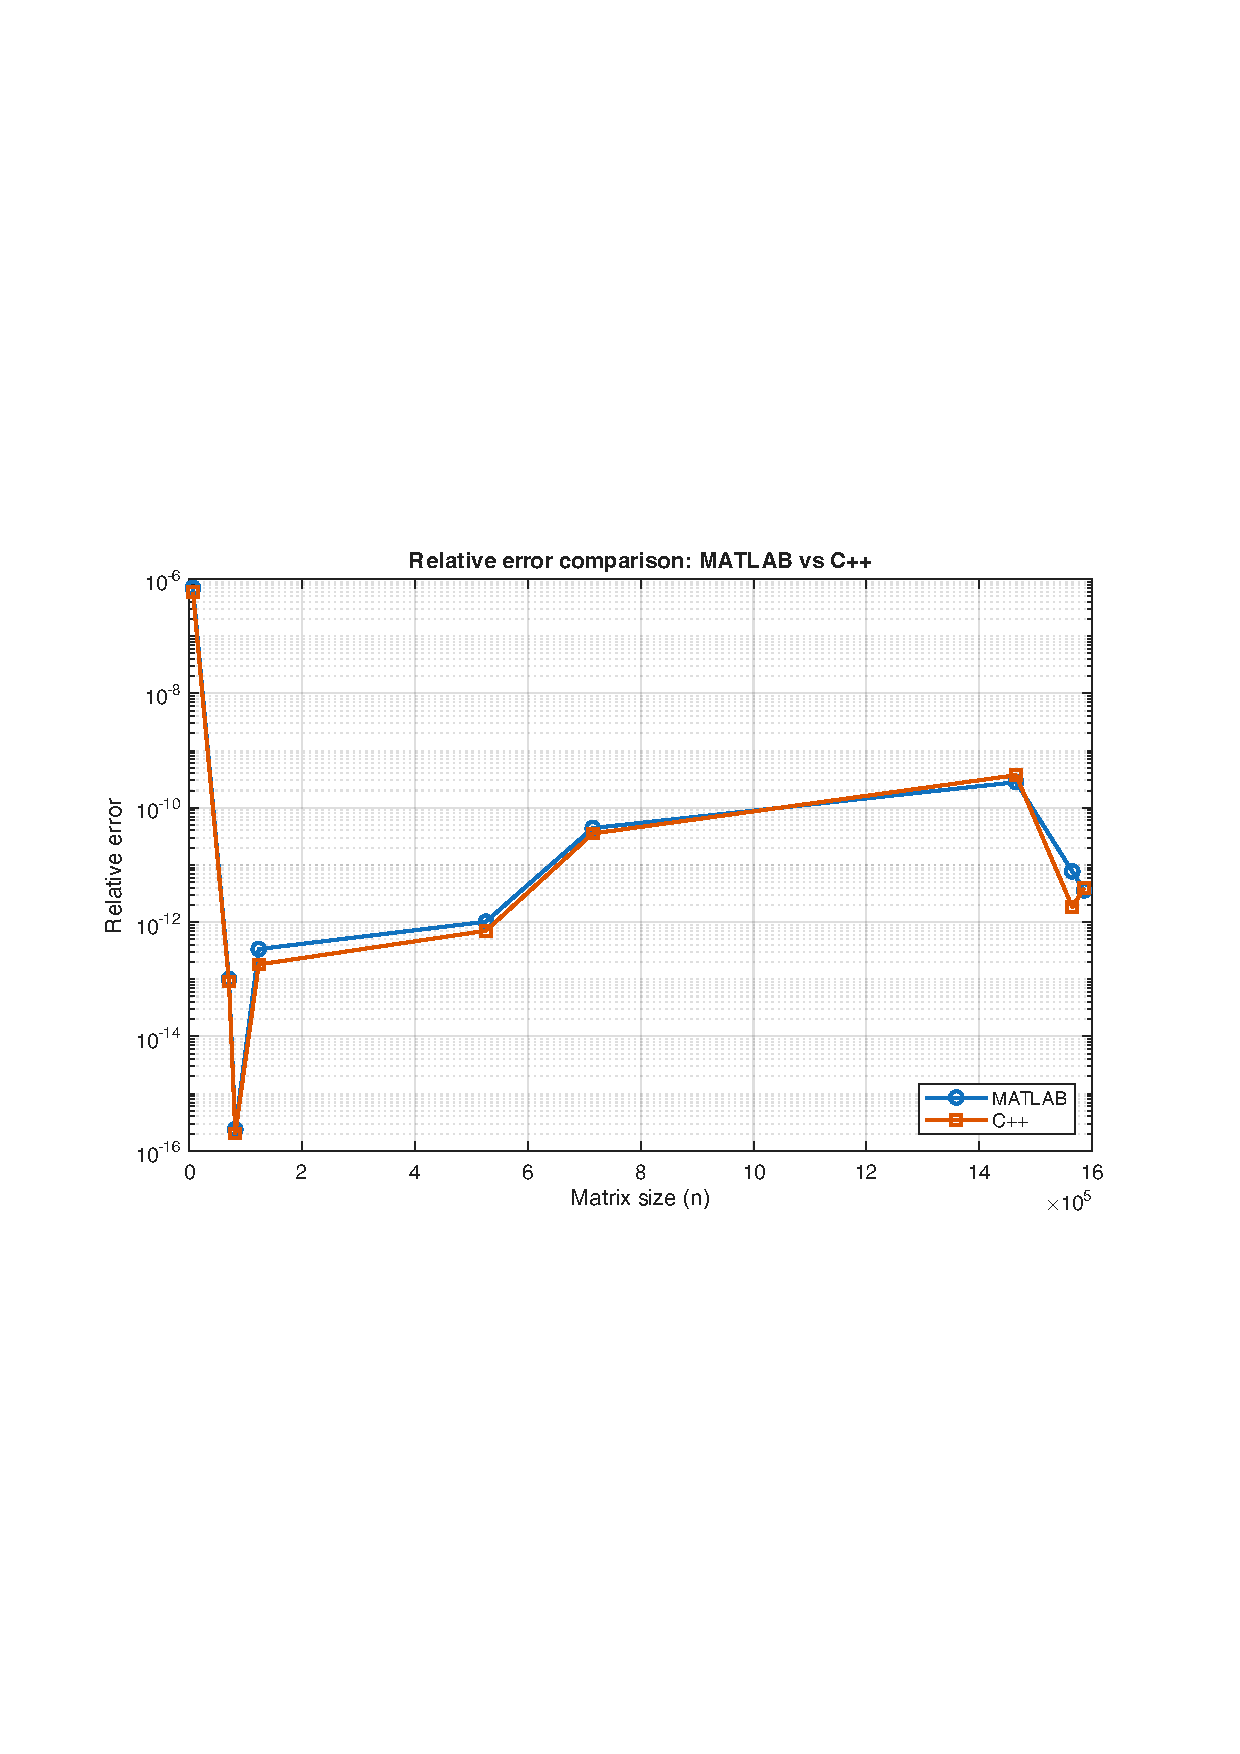
\includegraphics[
        width=\textwidth,
        trim= 0cm 9cm 0cm 9cm,
        clip
    ]{../plots/comparison/windows/relative_error_comparison.pdf}
    \caption{Confronto degli errori relativi su Windows}
    \label{fig:windows_relerr}
\end{figure}
\begin{figure}[hbt]
    \centering
    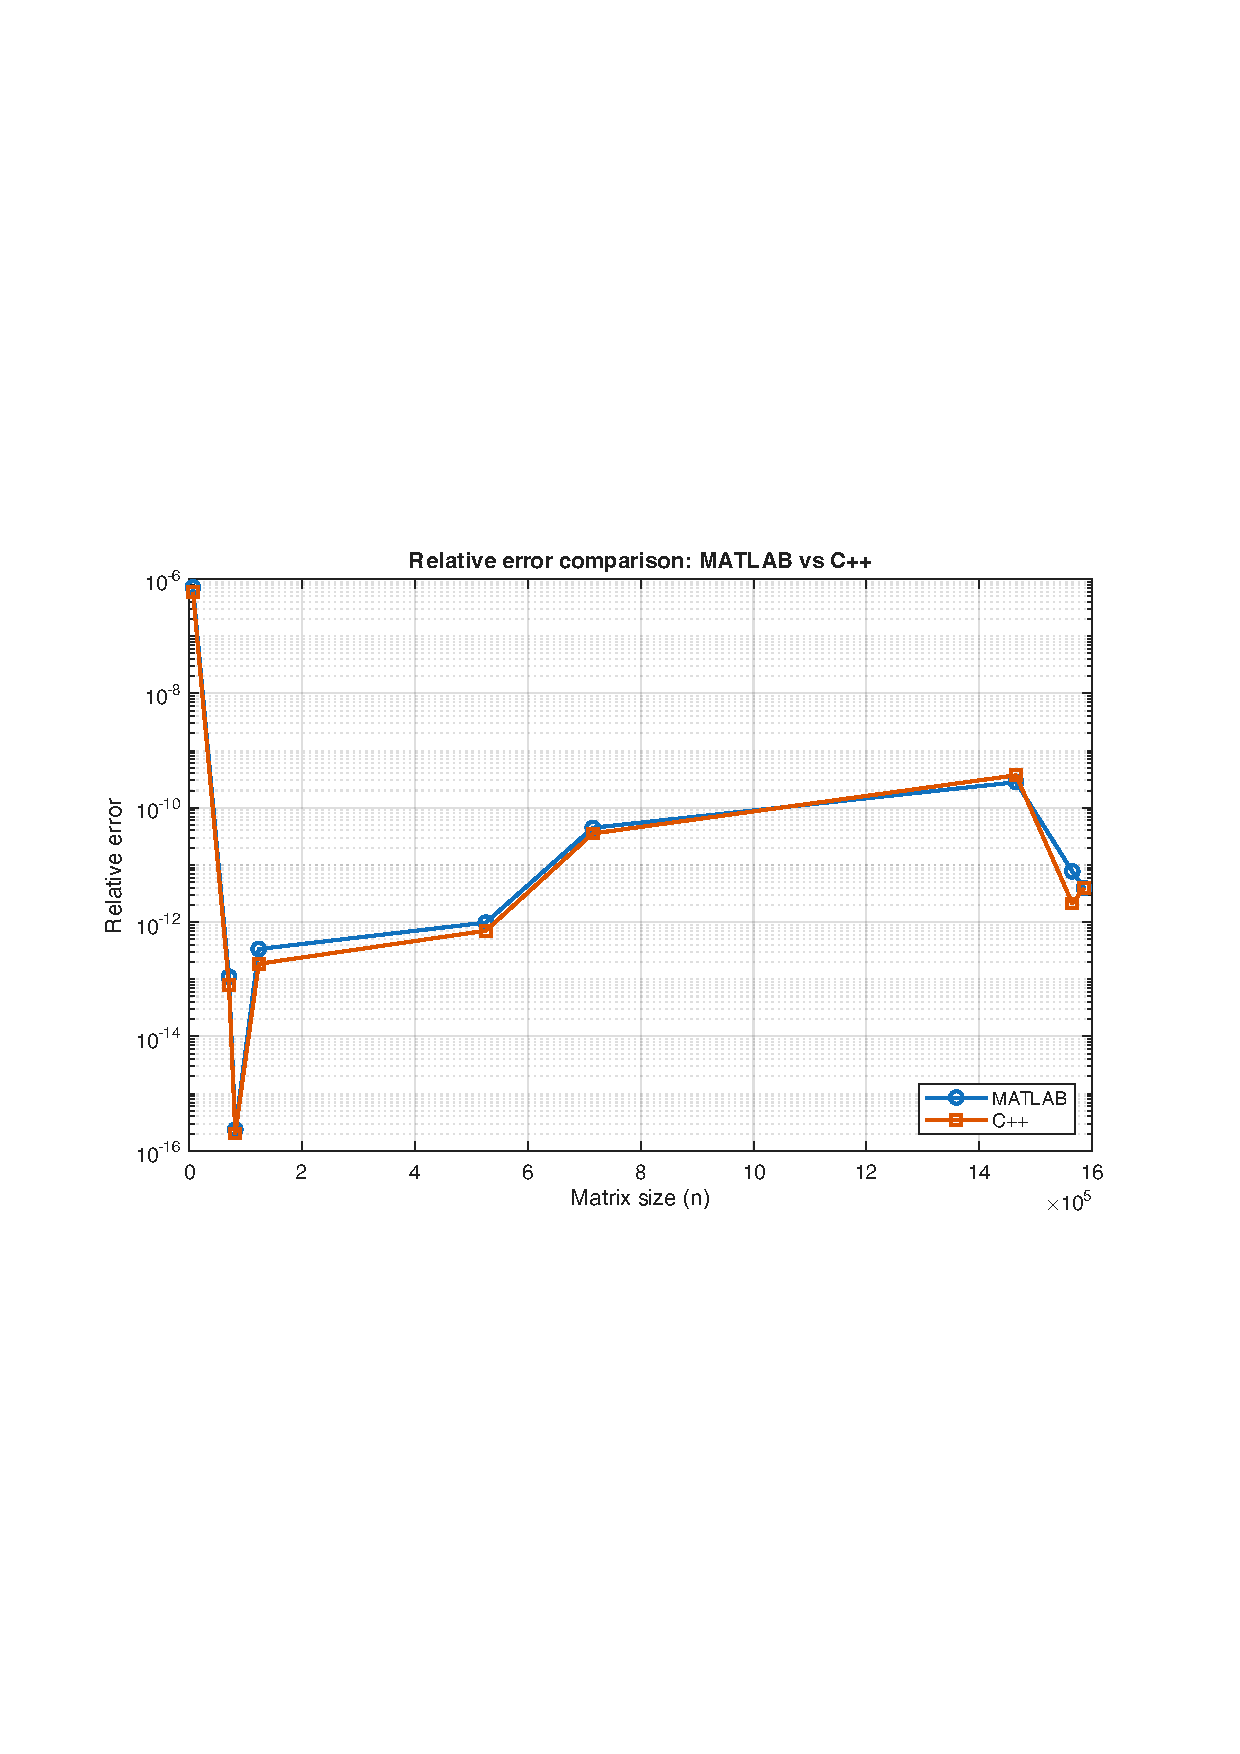
\includegraphics[
        width=\textwidth,
        trim= 0cm 9cm 0cm 9cm,
        clip
    ]{../plots/comparison/linux/relative_error_comparison.pdf}
    \caption{Confronto degli errori relativi su Linux}
    \label{fig:linux_relerr}
\end{figure}
\begin{figure}[H]
    \centering
    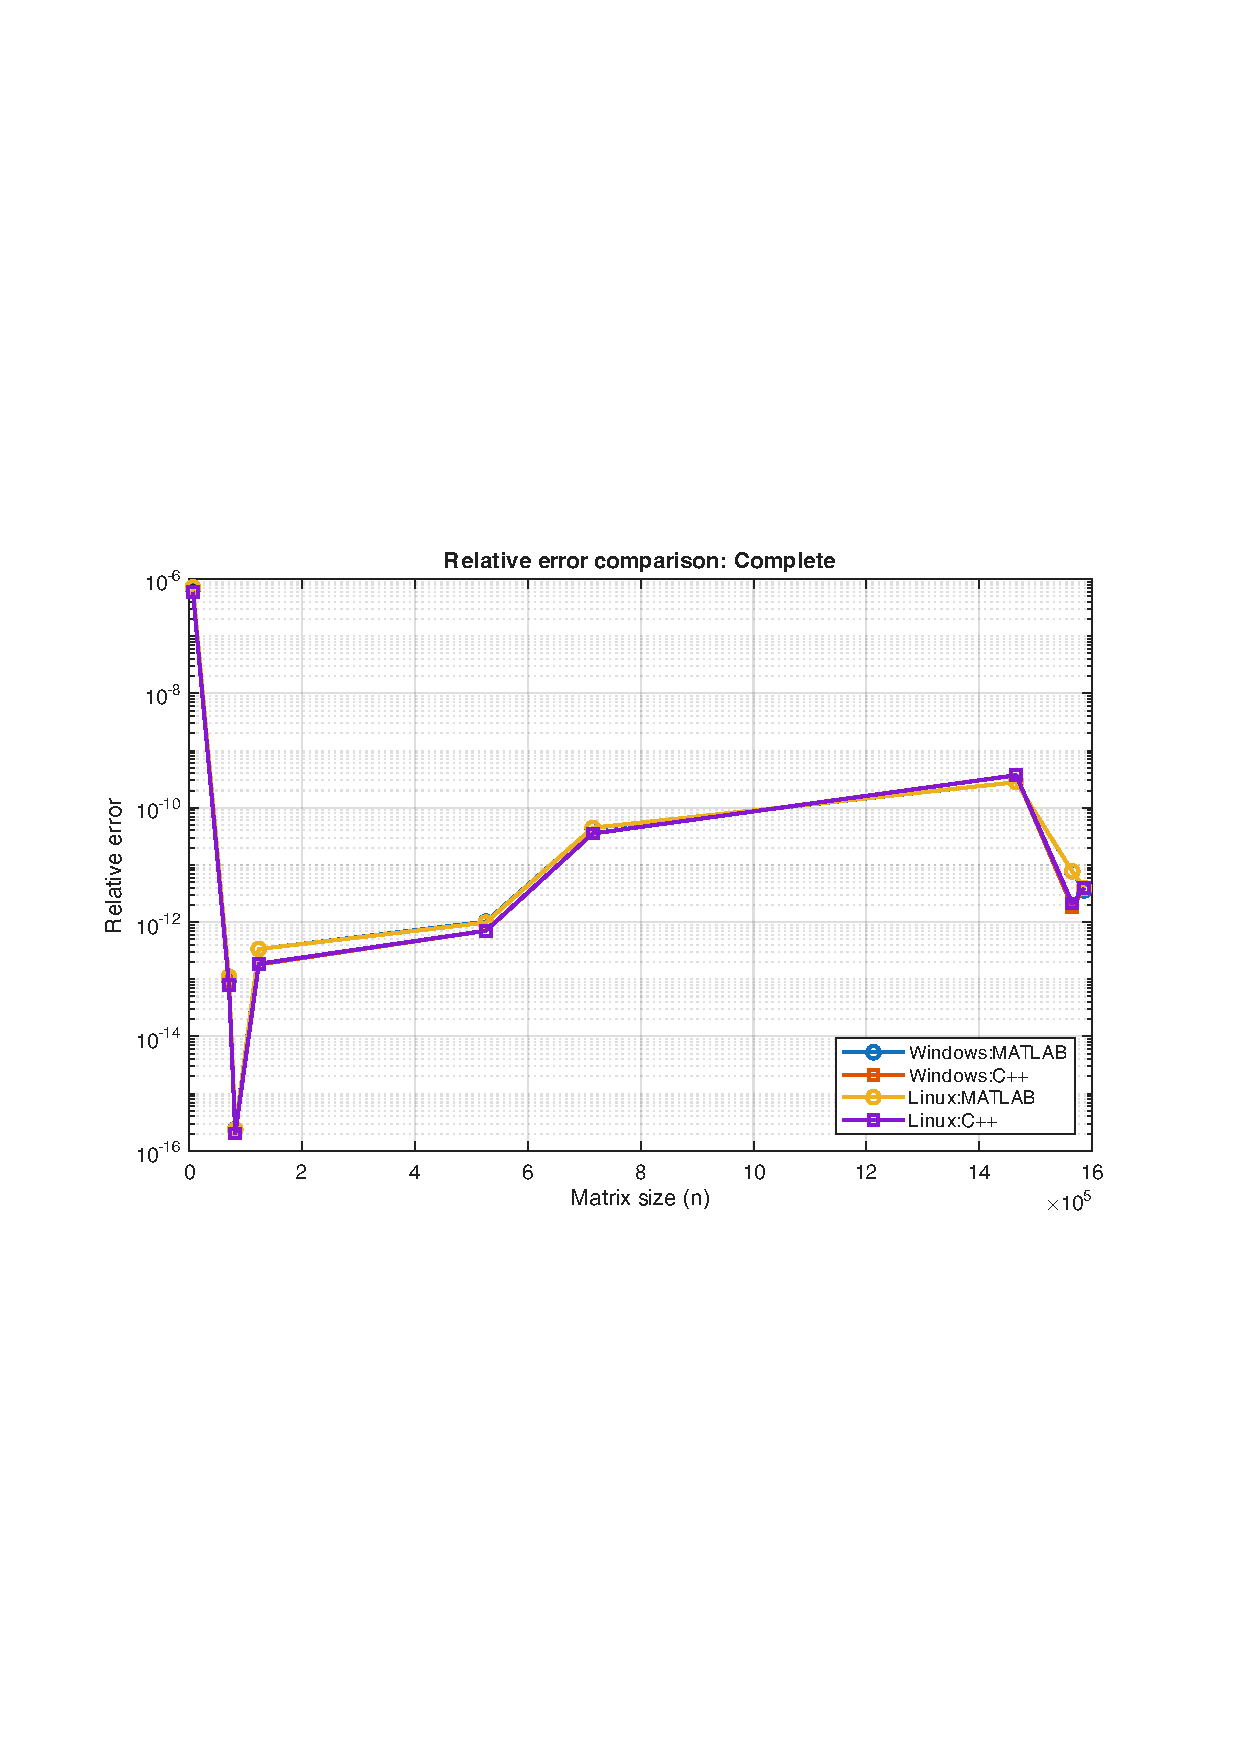
\includegraphics[
        width=\textwidth,
        trim= 0cm 9cm 0cm 9cm,
        clip
    ]{../plots/comparison/complete/relative_error_comparison.pdf}
    \caption{Confronto degli errori relativi su entrambi i sistemi operativi}
    \label{fig:complete_relerr}
\end{figure}
\chapter{Conclusioni}
In conclusione, i benchmark eseguiti hanno mostrato come entrambi gli ambienti analizzati, Matlab e C++,
siano in grado di risolvere sistemi lineari sparsi di grandi dimensioni tramite fattorizzazione di Cholesky.
Tuttavia, i risultati ottenuti evidenziano differenze significative in termini di prestazioni e gestione delle risorse.

Per quanto riguarda i tempi di esecuzione, il programma sviluppato in C++ ha mostrato performance generalmente migliori rispetto a Matlab, soprattutto all'aumentare delle dimensioni delle matrici.
Questo comportamento sulle matrici di dimensioni maggiori è dovuto principalmente all'assenza di swapping sul programma C++, che riesce a mantenere un utilizzo della memoria più contenuto durante la fase di fattorizzazione e risoluzione del sistema lineare.
Matlab, pur implementando internamente algoritmi altamente ottimizzati e sfruttando librerie numeriche avanzate, tende invece ad allocare quantità di memoria maggiori, causando operazioni di swapping per le matrici più pesanti e introducendo quindi un significativo overhead temporale.
Se fosse stato utilizzato un sistema con più memoria RAM, è possibile che le differenze di tempo tra i due programmi sarebbero risultate meno marcate.

Dal punto di vista dell'utilizzo della memoria, i risultati mostrano come il programma C++ occupi mediamente meno spazio rispetto a Matlab per le matrici di dimensioni più elevate.
Le differenze osservate per matrici di ordine inferiore risultano invece influenzate sia dai diversi formati utilizzati per la rappresentazione delle matrici sia dalle differenti strategie di gestione della memoria adottate dai due ambienti.
Inoltre, la presenza dello swapping rende difficile effettuare un confronto perfettamente accurato della memoria realmente utilizzata da Matlab nei casi più estremi.

Per quanto riguarda la precisione numerica, le differenze osservate tra Matlab e C++ risultano marginali e dipendono principalmente dalle specifiche implementazioni dei solver e delle librerie utilizzate.
In particolare, il solver basato su CHOLMOD integrato in Eigen ha mostrato, nella maggior parte dei casi, errori relativi leggermente inferiori rispetto a quelli ottenuti con Matlab.
\section{Usabilità}
Dal punto di vista dell'usabilità, Matlab offre un ambiente significativamente più immediato e semplice da utilizzare rispetto a C++.
La presenza di funzionalità integrate per l'algebra lineare,
gestione automatica della memoria e una sintassi ad alto livello permette infatti di sviluppare rapidamente programmi numerici complessi con una quantità ridotta di codice.
Al contrario, lo sviluppo dell'applicazione in C++ ha richiesto una gestione esplicita delle dipendenze,
la configurazione dell'ambiente di build e l'integrazione manuale di librerie esterne.

In particolare, l'installazione e la configurazione dell'ambiente C++ su Windows si sono rivelate significativamente più complesse rispetto a Matlab.
La necessità di compilare manualmente librerie come SuiteSparse e OpenBLAS con supporto al multithreading,
configurare correttamente CMake e gestire le dipendenze tramite strumenti esterni ha reso il setup più articolato e soggetto a problematiche di compatibilità.
Matlab, invece, mette a disposizione un ecosistema già integrato e pronto all'uso,
nel quale la maggior parte delle funzionalità necessarie è immediatamente disponibile senza ulteriori configurazioni.
\section{Documentazione}
Per quanto riguarda la documentazione, entrambi gli ambienti risultano ben supportati, ma con differenze sostanziali nell'approccio.
Matlab dispone di una documentazione centralizzata, uniforme e facilmente consultabile, particolarmente adatta ad un utilizzo didattico e introduttivo, tuttavia è limitata nei dettagli implementativi in quanto closed source.
L'ambiente C++, invece, richiede la consultazione della documentazione di molteplici librerie distinte, spesso con livelli di dettaglio e qualità differenti.
Tuttavia, librerie mature come Eigen e CHOLMOD mettono a disposizione documentazioni tecniche estremamente approfondite,
che permettono un elevato livello di controllo e ottimizzazione dell'applicazione.

\section{Confronto finale}
Complessivamente, i risultati ottenuti evidenziano come un'implementazione sviluppata in C++,
opportunamente ottimizzata e supportata da librerie numeriche specializzate come Eigen, SuiteSparse e OpenBLAS,
possa offrire prestazioni superiori rispetto a Matlab sia in termini di tempo di esecuzione sia di utilizzo della memoria.
Matlab rimane comunque uno strumento estremamente efficace per lo sviluppo rapido e per la prototipazione di algoritmi numerici,
grazie alla semplicità d'uso, all'elevato livello di astrazione e alla disponibilità di strumenti integrati avanzati.

Si può quindi concludere che Matlab rappresenti una soluzione più accessibile,
semplice da configurare e particolarmente adatta alla prototipazione rapida,
mentre C++ costituisce una scelta più complessa dal punto di vista implementativo,
ma capace di offrire maggiore controllo sull'hardware
e migliori prestazioni complessive nei casi di calcolo numerico intensivo.
Nel caso ipotetico presentato nella traccia, se si ha a disposizione del personale esperto in C++,
questo risulta la scelta migliore in particolare su piattaforma Linux,
dove la gestione delle dipendenze è molto più semplice.
Dove questo non è possibile, Matlab rappresenta comunque una valida alternativa,
soprattutto se si dispone di un sistema con sufficiente memoria RAM per evitare problemi di swapping,
tenendo presente tuttavia del costo elevato delle licenze.
Per Matlab, l'installazione risulta molto più semplice e rapida su Windows,
mentre su Linux è necessario utilizzare un gestore di pacchetti dedicato o seguire procedure più complesse per l'installazione.
Inoltre, molte distribuzioni Linux non sono ufficialmente supportate da Matlab.


\printbibliography

\end{document}